\documentclass[12pt,a4paper]{report}

% --- Paquetes de Idioma y Codificación ---
\usepackage[utf8]{inputenc}
\usepackage[T1]{fontenc}
\usepackage[spanish, es-tabla]{babel}

% --- Diseño de Página ---
\usepackage{geometry}
\geometry{top=2.5cm, bottom=2.5cm, left=3cm, right=3cm}

% --- Matemáticas y Símbolos ---
\usepackage{amsmath, amssymb, amsthm}

% --- Colores y Cajas ---
\usepackage[dvipsnames]{xcolor}
\usepackage[most]{tcolorbox}

% Caption

\usepackage{caption}

% Gráficos

\usepackage{graphicx}

% Espaciadora

\newcommand{\esp}{\vspace{0.5cm}}

% promedio

\newcommand{\prom}[1]{\left\langle #1 \right\rangle}

% ket

\newcommand{\ket}[1]{| #1 \rangle}

% bra

\newcommand{\bra}[1]{\langle #1 |}

% braket

\newcommand{\braket}[2]{\langle #1 | #2 \rangle}

% Bibliografía

\usepackage[style=apa, backend=biber]{biblatex} % Estilo APA
\addbibresource{biblio.bib} % Nombre de tu archivo .bib

% Configuración de cajas personalizadas
\newtcolorbox{importante}{
	colback=red!5!white,
	colframe=red!75!black,
	title=Importante,
	fonttitle=\bfseries
}

\newtcolorbox{nota}{
	colback=blue!5!white,
	colframe=blue!75!black,
	title=Nota,
	fonttitle=\bfseries
}

% Definición de la caja de bibliografía
\newtcolorbox{bibliografia}{
	colback=gray!5!white,
	colframe=gray!75!black,
	title=Bibliografías útiles,
	fonttitle=\bfseries,
	breakable
}

% Socrative para óptica 2

\newtcolorbox{Socrative}{
	colback=orange!5!white,
	colframe=orange!75!black,
	title=Socrative,
	fonttitle=\bfseries,
	breakable
}

% Float

\usepackage{float}

% --- Hipervínculos ---
\usepackage{hyperref}
\hypersetup{
	colorlinks=true,
	linkcolor=blue,
	filecolor=magenta,      
	urlcolor=cyan,
}

% --- Datos del Documento ---
\title{Óptica II}
\author{Chengyu Jin}
\date{\today}

\begin{document}
	
	\maketitle
	
	\tableofcontents
	\newpage
	
	\chapter{ Interacción luz-materia. Modelo clásico}
	
	\section{Introducción}
	
	\begin{figure}[H]
		\centering
		\includegraphics[width=0.7\textwidth]{IMG/intro1.png}
	\end{figure}
	
	\esp
	
	Hasta ahora, hemos estudiado principalmente dos tipos de fenómenos en relación a la naturaleza ondulatoria de la luz: los que podemos agrupar como de interacción luz-luz (interferencias, difracción, polarización) y los de propagación (en medios isótropos, metales y anisótropos). Pero hay una serie de fenómenos que hemos dejado fuera de la descripción teórica o bien los hemos tratado de forma muy incompleta. Se refieren a la interacción entre la luz y la materia por la cual se propaga, que hasta ahora hemos ignorado (aunque la propagación es en cierta medida un fenómeno de interacción también). 
	
	\esp
	
	En nuestro modelo de propagación para medios homogéneos e isótropos, hemos asumido que en el medio había una serie de constantes que regulaban la interacción con las ondas e.m., como la constante dieléctrica $\epsilon$, la permeabilidad magnética $\mu$ y la conductividad $\sigma$. Pero no hemos considerado en nuestro tratamiento (aunque sí lo hemos mencionado en ocasiones) la dependencia de estas constantes con las características de la onda e.m. incidente en el medio.
	
	\esp
	
	\begin{figure}[H]
		\centering
		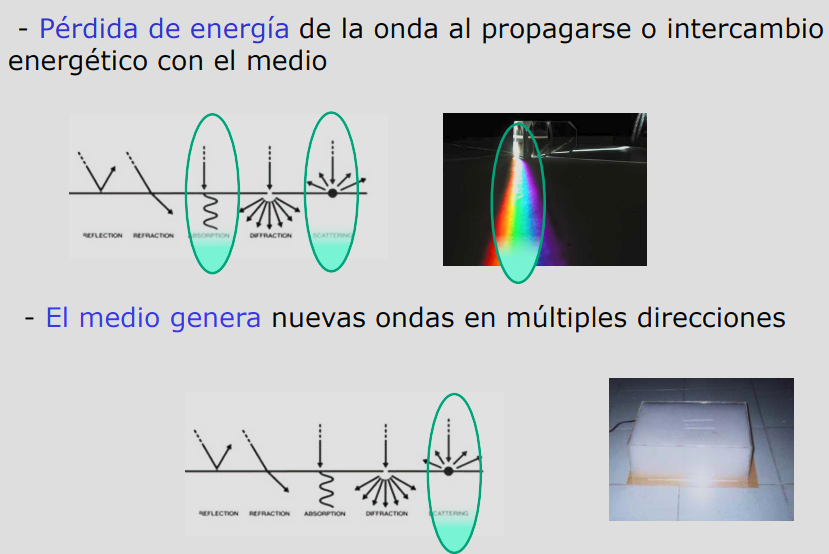
\includegraphics[width=0.7\textwidth]{IMG/Intro3.png}
	\end{figure}
	
	\esp
	
	Esto resulta fundamental para explicar una serie de fenómenos que suponen transferencia de energía entre la onda y el medio, como la absorción, y el esparcimiento, que hasta ahora no hemos abordado. El esparcimiento consiste en la re-emisión en todas direcciones de la energía incidente sobre una partícula en un medio material dado. Para entender la diferencia entre absorción y esparcimiento, podemos poner el ejemplo de una cubeta llena de humo sobre la que hacemos incidir luz blanca de la cubeta, vemos que ha disminuido apreciablemente. Esta disminución se debe a una combinación de absorción por las partículas sólidas del humo (en este caso, la energía se disipa), y de esparcimiento de la luz incidente por dichas partículas (en cuyo caso, la luz se re-emite en muchas direcciones, y podemos verla si miramos la cubeta desde uno de sus lados).
	
	\esp
	
	La absorción selectiva también se relaciona con los espectros de emisión de las fuentes de descarga de gases, y en último término con las longitudes de onda que son reflejadas preferentemente por un objeto, determinando su color.
	
	\esp
	
	\begin{figure}[H]
		\centering
		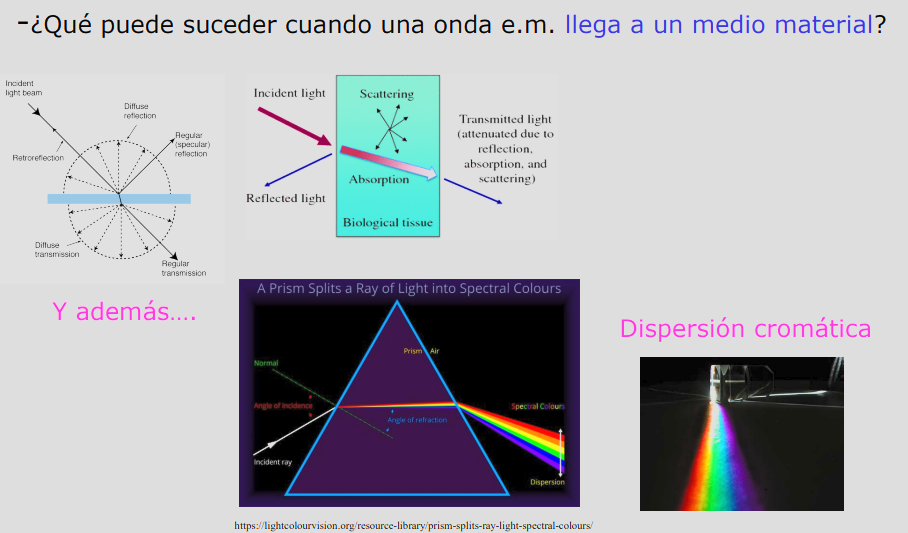
\includegraphics[width=0.7\textwidth]{IMG/Intro2.png}
	\end{figure}
	
	\esp
	
	Por otra parte, hay fenómenos que quedan perfectamente descritos con el marco teórico utilizado hasta ahora, que son los que \textbf{no suponen intercambio energético} ni cambios de frecuencia en la onda incidente, por ejemplo la refracción y la reflexión. En cuanto a la propagación, queda explicada de forma muy imperfecta si no abordamos la dependencia del índice de refracción con la frecuencia de la radiación incidente, que se relaciona con los fenómenos de dispersión cromática que hemos tratado de forma no completa en Óptica I. En definitiva, necesitamos un nuevo modelo que complete la descripción puramente ondulatoria de la luz. Dejamos todavía fuera muchos fenómenos de interacción luz-materia a nivel atómico, que serían objeto de la óptica cuántica (efectos fotoeléctrico y Compton, por ejemplo). De momento, vamos a utilizar una descripción clásica, no un modelo cuántico. Mantenemos el modelo de luz como onda e.m., y de materia como un conjunto de unidades atómicas formadas por distribuciones de partículas cargadas (electrodinámica clásica).
	
	\esp
	
	\begin{figure}[H]
		\centering
		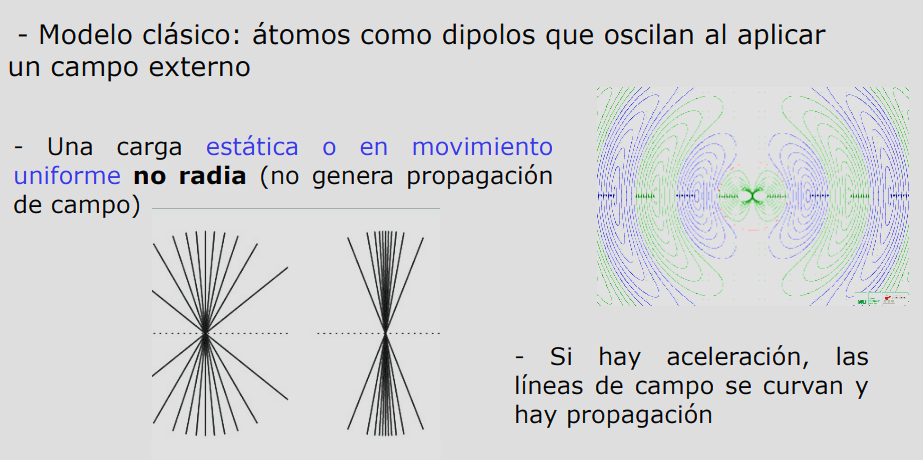
\includegraphics[width=0.7\textwidth]{IMG/Intro4.png}
	\end{figure}
	
	\esp
	
	Nos basaremos en un modelo de los átomos que forman la materia que los considera como un conjunto de dipolos oscilantes que pueden producir o absorber radiación. Una idea inicial básica de este modelo, que debemos repasar, es que una carga libre (no ligada a un átomo) en reposo o que se mueve con movimiento uniforme (velocidad constante) \textbf{no produce radiación}, puesto que genera un campo eléctrico $\vec{E}$ constante, y no genera campo magnético asociado. El caso de movimiento uniforme se explica pensando que, si tomamos el sistema de referencia relativo que se desplaza con la carga, ésta estaría en reposo en dicho sistema, y por tanto tendría las mismas propiedades que en el sistema inicial de la carga que no se mueve en cuanto a la emisión de energía. Mirando la carga libre desde el sistema en reposo, tendríamos un campo $\vec{E}$ constante y un campo magnético $\vec{B}$ asociado con líneas cerradas circulares, pero dado que las líneas de campo eléctrico serían rectas (asociadas al movimiento de la carga, porque el campo no está disociado de la misma), \textbf{entonces no puede generarse radiación}. La diferencia entre ambas situaciones estaría en la uniformidad de las líneas de campo, que puede despreciarse salvo para velocidades muy elevadas de la carga. 
	
	\esp
	
	Sin embargo, si la carga sufre una aceleración, entonces sí que emite o \textbf{intercambia radiación} puesto que las líneas de campo ya no son rectas sino curvas. Esto es precisamente el fundamento de la emisión de algunas fuentes de radiación, como el láser de electrones libres (FEL) o la radiación sincrotrón [1]. El fundamento de esta emisión se describe en [1] aplicado al caso de la radiación de frenado. El cambio irregular en la posición de la carga y la necesidad de que las líneas de campo estén siempre conectadas hace que se creen variaciones rápidas de orientación en las líneas de campo eléctrico, y por tanto componentes transversales del mismo que se van propagando hacia fuera como un pulso. Este campo eléctrico variable generará a su vez un campo magnético, y la onda resultante llevará asociada energía que se propaga en todas direcciones menos en la de movimiento de la carga.
	
	\section{El átomo como dipolo oscilante (modelo de Lorentz)}
	
	\begin{figure}[H]
		\centering
		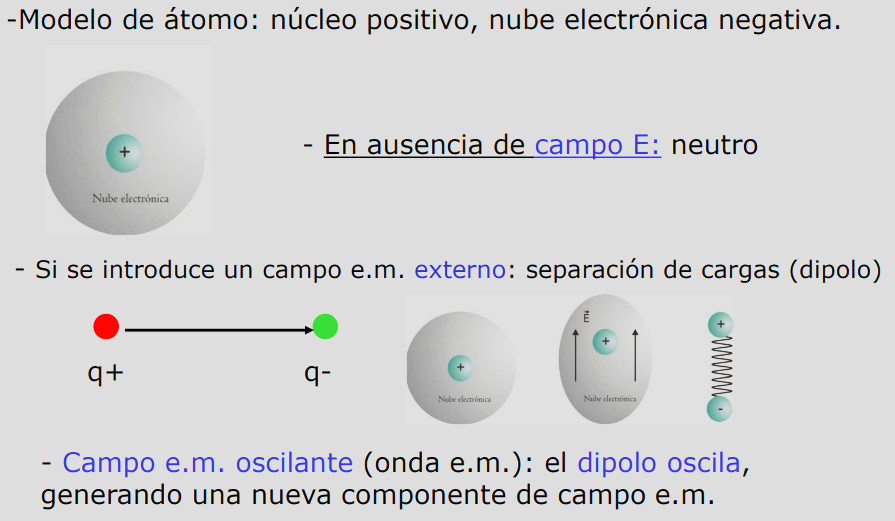
\includegraphics[width=0.7\textwidth]{IMG/lorentz.png}
	\end{figure}
	
	\esp
	
	El modelo de átomo que vamos a considerar consiste en una asociación de partículas cargadas positivamente o neutras que forman el núcleo, y una nube de electrones alrededor, de forma que la carga negativa global iguala a la positiva global (sistema neutro en equilibrio). Si introducimos un campo e.m. externo, se produce una polarización o separación de las cargas positivas y negativas, y el átomo pasa a poder ser considerado o descrito como un dipolo. Si el campo e.m. vibra (onda e.m.), el dipolo oscila a su vez, generando una nueva componente de campo e.m. (onda e.m. que a su vez se propaga por el medio que contiene al dipolo).
	
	\esp
	
	\begin{figure}[H]
		\centering
		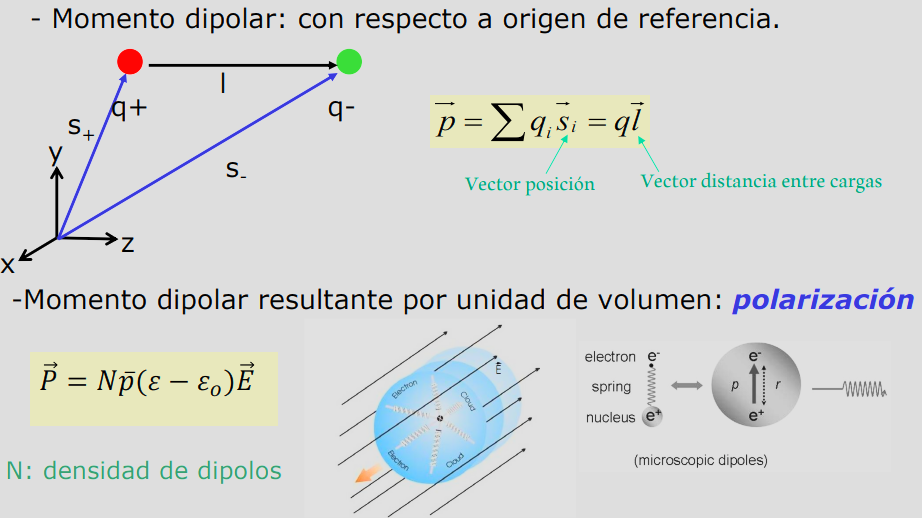
\includegraphics[width=0.7\textwidth]{IMG/lorentz2.png}
	\end{figure}
	
	\esp
	
	Vamos a verlo un poco más despacio. Cualquier dipolo puede caracterizarse por su momento dipolar con respecto a un sistema de referencia dado, definido como el producto de las cargas por sus respectivos vectores de posición. En el caso de nuestro dipolo atómico, la carga negativa iguala a la positiva, con lo cual el momento dipolar queda en función del vector distancia entre cargas, como vemos en la figura.

	\esp
	
	\begin{figure}[H]
		\centering
		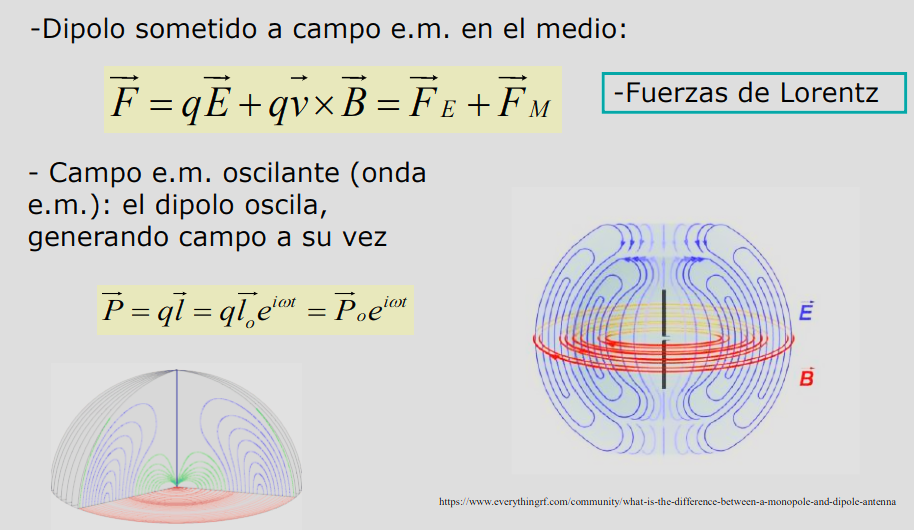
\includegraphics[width=0.7\textwidth]{IMG/lorentz3.png}
	\end{figure}
	
	\esp
	
	Definimos la polarización como el momento dipolar resultante por unidad de volumen, y como recordamos de temas anteriores, es proporcional al campo $\vec{E}$ aplicado ($\vec{P} = (\epsilon - \epsilon_o)\vec{E}$). Si el dipolo se somete a un campo e.m., experimenta, según nuestro modelo clásico, la acción de las fuerzas de Lorentz, con dos componentes: eléctrica y magnética. La componente eléctrica sería $\vec{F} = q_e \vec{E}$. Para velocidades muy elevadas, habría que aplicar las expresiones correspondientes a electrodinámica relativista, pero para los fenómenos que vamos a tratar, las velocidades son bajas y no van a requerir este tratamiento.
	
	\esp
	
	Si el campo e.m. es armónico (onda e.m.), el dipolo oscila (la distancia entre las cargas se acorta y se alarga periódicamente), con lo cual se genera una componente de campo e.m., como vemos en la figura, que se va propagando según va oscilando el dipolo, pero no por igual en todas direcciones. El momento dipolar podrá expresarse como una función armónica que depende del momento dipolar máximo y de la frecuencia de oscilación $\omega$.
	
	\begin{equation*}
		\vec{P} = \vec{P}_o e^{i\omega t}
	\end{equation*}
	
	A una distancia del centro del dipolo $r$, grande con respecto a la separación máxima entre cargas, la configuración del campo e.m. emitido es simple, con el vector $\vec{E}$ contenido en el plano que forman el dipolo y el vector $\vec{r}$, y el campo magnético $\vec{H}$ perpendicular a $\vec{E}$, como vemos en la figura.
	
	\esp
	
	\begin{figure}[H]
		\centering
		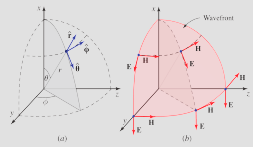
\includegraphics[width=0.4\textwidth]{IMG/fig.png}
	\end{figure}
	
	\esp
	
	\begin{figure}[H]
		\centering
		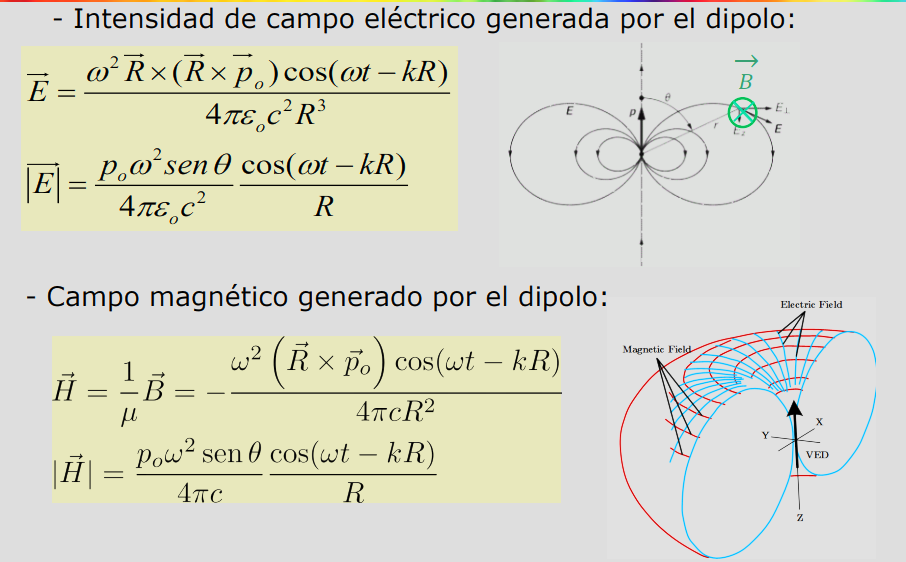
\includegraphics[width=0.7\textwidth]{IMG/lorentz4.png}
	\end{figure}
	
	\esp
	
	La dirección de la propagación de energía es entonces radial desde el dipolo (vector de Poynting $\vec{M}$). Puede demostrarse (ver [3] p. 368) la dependencia del módulo del vector campo eléctrico con el momento dipolar máximo y el ángulo que forma la dirección de propagación con el eje del dipolo (ángulo $\theta$).
	
	\begin{equation*}
		E = \frac{p_o \omega^2 \sin \theta \cos(kr - \omega t)}{4\pi \epsilon_o r}
	\end{equation*}
	
	\esp
	
	\begin{figure}[H]
		\centering
		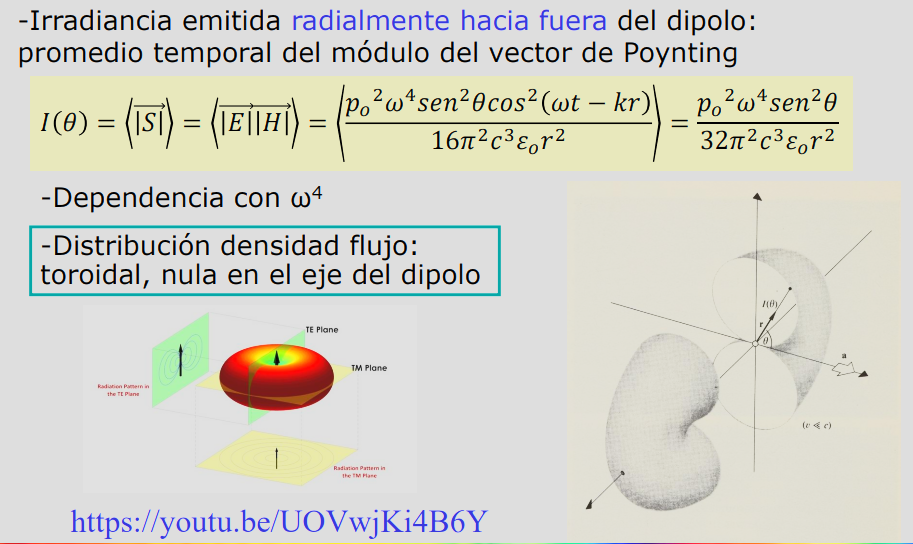
\includegraphics[width=0.7\textwidth]{IMG/lorentz5.png}
	\end{figure}
	
	\esp
	
	La irradiancia emitida radialmente (módulo del vector de Poynting) resulta dependiente de la cuarta potencia de la frecuencia de vibración del dipolo, y al igual que el campo $\vec{E}$, es nula en la dirección del dipolo y máxima y constante en el ecuador de la esfera de propagación (plano perpendicular al dipolo que pasa por su punto medio). En tres dimensiones, tenemos una distribución toroidal de campo, como se observa en la figura.
	
	\begin{equation*}
		I(\theta, r) = \frac{c\epsilon_o}{2} E^2 = \frac{p_o^2 \omega^4 \sin^2 \theta}{32 \pi^2 c^3 \epsilon_o r^2}
	\end{equation*}
	
	\esp
	
	Este fenómeno está relacionado con la radiación sincrotrón que hemos mencionado en el primer apartado ([1]). La dependencia con la cuarta potencia de la frecuencia indica que la radiación es más intensa conforme mayor sea la frecuencia de oscilación del dipolo.
	
	\esp
	
	\begin{figure}[H]
		\centering
		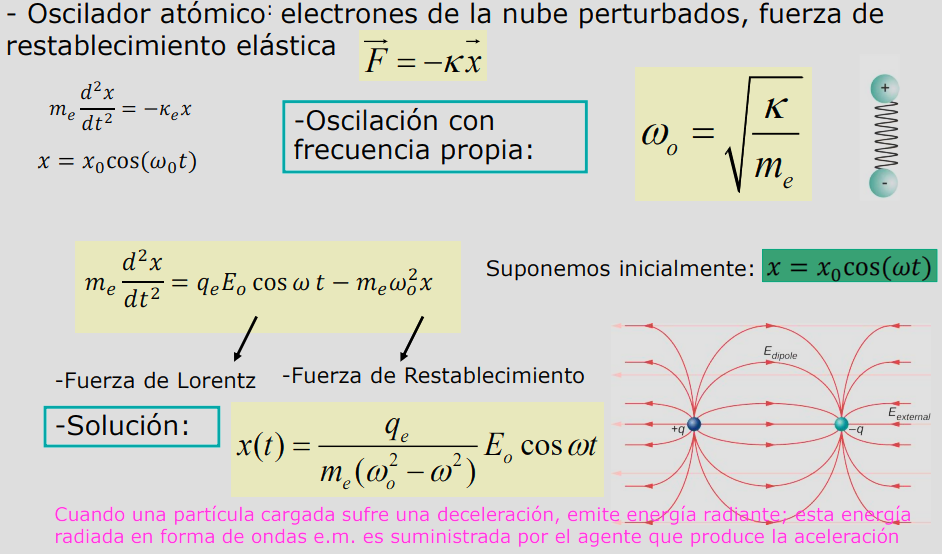
\includegraphics[width=0.7\textwidth]{IMG/lorentz6.png}
	\end{figure}
	
	\esp
	
	Hemos obtenido la irradiancia radiada por el dipolo, pero hasta ahora no hemos caracterizado la variación de la distancia entre cargas para un oscilador atómico (es decir, cómo varía la separación entre núcleo y nube electrónica, según nuestro modelo). Para esto, vamos a resolver la ecuación de dinámica del movimiento armónico correspondiente. Visualizamos el átomo como un sistema ligado, es decir, que hay una fuerza de atracción que mantiene el sistema en equilibrio e impide la dispersión de las cargas. Si el átomo resulta perturbado, como ocurre cuando incide una onda e.m. en el medio, resulta plausible suponer que hay una fuerza de equilibrio tendente a oponerse a la perturbación y restablecer el equilibrio del sistema, a la que llamamos fuerza de restablecimiento. Resulta proporcional a la separación entre núcleo y nube, por lo que adopta la forma de la Ley de Hooke $\vec{F} = -k\vec{x}$. Si un electrón es sometido sólo a esta fuerza de restablecimiento, oscilará en torno a su posición de equilibrio con una frecuencia (que denominamos frecuencia propia) $\omega_o$. Esta frecuencia es inversamente proporcional a la masa del electrón. Si añadimos la perturbación de una onda e.m., con su fuerza de Lorentz eléctrica correspondiente, cada átomo se comporta como un oscilador forzado clásico, cuya ecuación se obtiene aplicando la segunda ley de Newton, y depende de la fuerza de Lorentz y la fuerza de restablecimiento.
	
	\begin{equation*}
		m_e \frac{d^2x}{dt^2} = q_e E_o \cos \omega t - m_e \omega_o^2 x
	\end{equation*}
	
	Resolviendo la ecuación, obtenemos la expresión para la distancia núcleo-nube, que como vemos vibra a la misma frecuencia de la radiación incidente y en fase con ella.
	
	\begin{equation*}
		x(t) = \frac{q_e}{m_e (\omega_o^2 - \omega^2)} E_o \cos \omega t
	\end{equation*}
	
	\noindent Como conclusiones de este modelo clásico, tenemos entonces:
	
	\begin{itemize}
		\item que el átomo sin fuerza impulsora vibra a frecuencia propia $\omega_o$.
		\item Que si la frecuencia de la onda incidente es menor que la propia, el oscilador sigue a la fuerza aplicada.
		\item Si la frecuencia incidente es mayor que la propia, la oscilación se opone a la fuerza impulsora.
	\end{itemize}
	
	Vamos ahora a aplicar este modelo (con alguna complicación adicional) a la descripción de fenómenos que implican intercambio energético de la onda incidente con el medio.

	\printbibliography[title={Bibliografía}]
\end{document}